% Derived from projects/eos/trunk/ds13.tex.  Another good source might
% be projects/like9501/xcp8_1_14
\documentclass{beamer}
\setbeamertemplate{navigation symbols}{} %no nav symbols
\usepackage{amsmath,amsfonts}
\usepackage[pdftex]{rotating}
\newcommand\logx{y}
\newcommand\logf{g}
\newcommand\Logf{G}
\newcommand{\argmin}{\operatorname*{argmin}}
\newcommand{\La}{{\cal L}}
\newcommand{\C}{{\cal C}}
\newcommand{\normal}[2]{{\cal N}(#1,#2)}
\newcommand{\COST}{\cal C}
\newcommand{\LL}{{\cal L}}
\newcommand{\X}{{\cal X}}
\newcommand{\PS}{{\cal P}}
\newcommand{\Prob}{\text{Prob}}
\newcommand{\field}[1]{\mathbb{#1}}
\newcommand{\EV}[2]{\field{E}_{#1}\left[#2\right]}
\newcommand\inner[2]{\left<#1,#2\right>}
\newcommand{\nomf}{\tilde f}
\newcommand\Polytope[1]{\field{P}_{#1}}
\newcommand\RN{\field{R}^{N}}
\newcommand\PolytopeN{\Polytope{N}}
\newcommand{\T}{{\cal P}}
\newcommand{\partialfixed}[3]{\left. \frac{\partial #1}{\partial #2}\right|_#3}
\newcommand\CJ[1]{{{#1}_{\text{CJ}}}}
\newcommand\dum{\xi}
\newcommand\Ddum{d\dum}

\title{Characterizing Uncertainty about Functions\footnote{LA-UR-17-22847}}

\author{Andy Fraser\footnote{Work with Stephen Andrews}}
\institute{Los Alamos National Laboratory}
\date{2017-4-21}

% \usetheme{Pittsburgh}
\usetheme{default}
\usefonttheme[]{serif}
\begin{document}
\frame{\titlepage
}

\frame{ \frametitle{Outline}\tableofcontents}

\section{The Motivating Example: EOS and a Nominal Isentrope}
\frame{
  \frametitle{Equations of State and Isentropes}

  \begin{columns}
    \begin{column}{0.6\textwidth}
      \resizebox{0.99\textwidth}{!}{\includegraphics{surf.pdf}}
    \end{column}
    \begin{column}{0.4\textwidth}
    \begin{align*}
      pv &= NRT & &\text{Ideal Gas} \\
      pv^\gamma &= c \\
      \gamma &\approx 3 & &\text{For our explosive}
    \end{align*}
    \end{column}
  \end{columns}
}

\section{A Toy Surrogate}
\frame{
  \frametitle{A Toy Surrogate}
  \begin{columns}
    \begin{column}{0.5\textwidth}
      \begin{center}
        \resizebox{0.99\textwidth}{!}{
          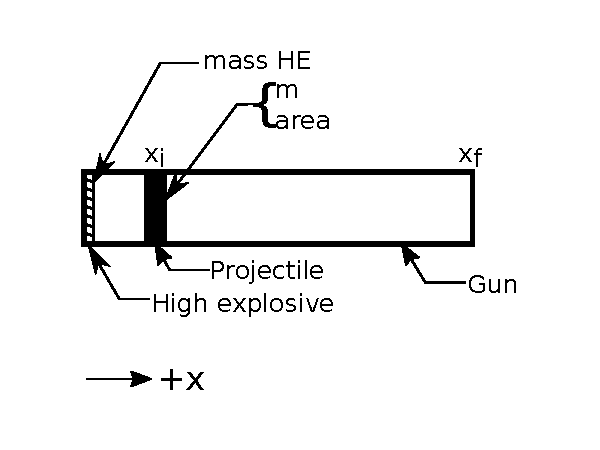
\includegraphics{static_figs/gun_poster.pdf}}
      \end{center}
    \end{column}
    \begin{column}{0.5\textwidth}
      \begin{center}
        \resizebox{0.99\textwidth}{!}{\includegraphics{figs/gun_tv.pdf}}
      \end{center}
    \end{column}
  \end{columns}
}

\section{Fisher Information}
\frame{
  \frametitle{Uncertainty and Fisher Information}
  After finding $\hat \theta \equiv \argmin_\theta C(\theta)$,
  characterize uncertainty by $\frac{\partial^2}{\partial \theta^2}
  C(\theta)$ or its expected value.  Note:
  \newcommand{\dmudtheta}{\left(\frac{\partial \mu_i(\theta)}
      {\partial \theta} \right)}
  \begin{equation*}
    \frac{\partial^2}{\partial \theta^2} \LL_i(\theta) = 
      \dmudtheta^T \Sigma_i^{-1} \dmudtheta +  (x_i-\mu_i(\theta))^T \Sigma_i^{-1}
       \left(\frac{\partial^2 \mu_i(\theta)}{\partial \theta^2} \right)
  \end{equation*}
  and since $\EV{x|\theta} x_i = \mu_i(\theta)$, the expected
  value of the second term is 0.  The first term, called the
  \emph{Fisher Information}
  \begin{equation*}
    {\cal{I}}(\theta)_i \equiv
    \EV{x|\theta}{\frac{\partial^2}{\partial \theta^2}
      \LL_i} = \dmudtheta^T \Sigma_i^{-1} \dmudtheta
  \end{equation*}
  characterizes how tightly the experiment constrains $\theta$.
}

\frame{
  \frametitle{Fisher Information for the Surrogate Problem}
  \begin{center}
    \resizebox{0.5\textwidth}{!}{\includegraphics{figs/gun_fisher.pdf}}
  \end{center}
}

\section{A Set of Convex Functions}
\frame{
  \frametitle{Expert Claim}

  \begin{columns}
    \begin{column}{0.4\textwidth}
      \resizebox{0.99\textwidth}{!}{\includegraphics{hixson.pdf}}
    \end{column}
    \begin{column}{0.19\textwidth}
      $p(v)$ is:\\
      Positive, \\
      Convex, \\
      $\hat p(v) \pm \frac{1}{2} \%$
    \end{column}
    \begin{column}{0.4\textwidth}
      \resizebox{0.99\textwidth}{!}{\includegraphics{lognom.pdf}}
    \end{column}
  \end{columns}
}

\section{Questions}
\frame{
  \frametitle{Questions}
  \begin{itemize}
  \item How do our numerical results depend on our choice of
    coordinates?
  \item Do limits exist that do not depend on coordinates?
  \item Is there a probability measure with measurable subsets for the
    region in function space specified by the Expert Claim?
  \end{itemize}

}

\frame{ \frametitle{Abstract}
  %
  We are fitting equations of state (EOS) to the mixtures of gasses
  produced by detonating explosives.  Given a set of experimental
  measurements, we intend our code to provide an estimate of the EOS
  and to characterize the residual uncertainty.  The presentation will
  outline the problem in sufficient detail to highlight key
  mathematical questions.
%
}

\end{document}

%%%---------------
%%% Local Variables:
%%% eval: (TeX-PDF-mode)
%%% End:
